%% ------------------------------------------------------------------------- %%
\chapter{Passeio de Euler}
\label{cap:passeio-euler}

\section{Introdução}

Agora que vimos um algoritmo eficiente que resolve o problema do \LCA\, vamos explorar uma outra técnica que tem mesmo tempo de complexidade. Entretanto, neste capítulo estudaremos um algoritmo capaz de resolver problemas um pouco mais complexos em que, por exemplo, é necessário atualizar o valor de um nó da árvore rapidamente (diferente dos outros algoritmos em que a árvore deveria ser sempre estática - isto é - sem modificações). No final deste capítulo será melhor explicado como isso pode ser útil e mostraremos uma aplicação prática.


\section{Descrição}

Vamos imaginar que, ao calcular o \LCA\ entre dois vértices distintos $a$ e $b$ temos uma função $F(x, y)$ que devolve todos os vértices no caminho de $a$ para $b$. Para melhor ilustrar isso, considere a seguinte árvore enraizada:

\vspace{0.5cm}

\begin{figure}[htb]
\begin{center}
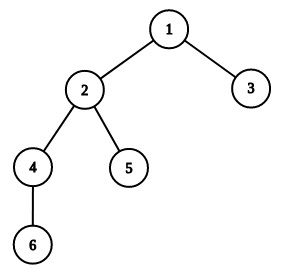
\includegraphics[width=6cm]{images/graph_euler.png}
\end{center}
\caption{\label{fig:arvore-euler}Árvore enraizada de 6 vértices}
\end{figure}

\vspace{0.5cm}

Assim, ao chamar $F(2, 3)$ a função nos retorna os vértices 2, 1 e 3.

Ao chamar $F(5, 6)$ os vértices devolvidos são 5, 2, 4 e 6.

Além disso, como de costume vamos também pré-calcular as profundidades de cada vértice de nossa árvore:

\begin{table}[htb]
\centering
\begin{tabular}{|l|c|c|c|c|c|c|}
\hline
Vértice      & 1 & 2 & 3 & 4 & 5 & 6  \\ \hline
Profundidade & 1 & 2 & 2 & 3 & 3 & 4 \\ \hline
\end{tabular}
\caption{Profundidades dos vértices da árvore acima}
\end{table}



Agora, para saber o \LCA\ entre dois nós $a$ e $b$, usaremos os vértices retornados pela chamada da função $F$ para eles (denotaremos o conjunto destes vértices de $V$). Afinal, pela definição o \LCA$(a, b)$ é o vértice menos profundo que contém $a$ e $b$ em sua subárvore. Isto é, o vértice menos profundo que está no caminho de $a$ até $b$.

Assim, basta verificar qual é o vértice de menor profundidade dentre os nós de $V$: no primeiro exemplo, tal vértice é 1 - enquanto no segundo exemplo é 2. Podemos verificar que eles são, de fato, os respectivos \LCA s de seus problemas.


\section{Obtendo todos os vértices de qualquer caminho}

Previamente assumimos que existe uma função F que retorna todos os vértices do caminho entre dois nós $a$ e $b$. Entretanto, ainda não estudamos como escrever esta função.

Toda vez que queremos fazer uma consulta entre dois vértices $a$ e $b$, poderíamos percorrer o caminho entre estes dois vértices de maneira bruta - o que geraria um gasto de tempo $O(n)$ para obter todos os vértices neste caminho.

Porém, podemos montar uma estrutura de dados que nos possibilita obter de maneira rápida todos os vértices no caminho entre quaisquer vértices $a$ e $b$.


\subsection{Passeio de Euler}

O que faremos é "planificar"\ uma árvore, de forma que tenhamos uma sequência de vértices em uma determinada ordem.

A ideia é visitar os vértices a partir da raiz contando o tempo em que passamos por um nó. A raiz, por exemplo, é visitada no tempo 1. Seu primeiro filho, no tempo 2. O primeiro filho de seu filho no tempo 3, e assim por diante. Assim, para cada vértice guardaremos:

\begin{itemize}
    \item Cada tempo em que aprofundamos a busca para um de seus filhos
    \item O tempo em que terminamos de aprofundar a busca em todos os seus filhos
\end{itemize}

Entender a ideia deste algoritmo é muito mais fácil com um exemplo. Para isso, usaremos novamente a árvore introduzida no início deste capítulo, já com os tempos que cada vértice guardou após a execução do Passeio de Euler:

\vspace{10cm}

\begin{figure}[htb]
\begin{center}
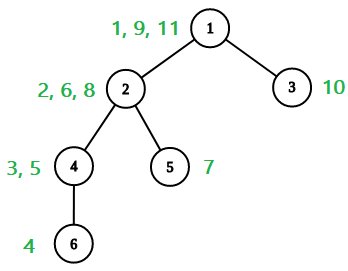
\includegraphics[width=6cm]{images/graph_euler_numbered.png}
\end{center}
\caption{\label{fig:arvore-euler2}Passeio de Euler na árvore}
\end{figure}

O código que gera os tempos de cada vértice é basicamente uma simples DFS:

Agora, ao fazer uma consulta nessa estrutura para os vértices $4$ e $5$, por exemplo, basta pegar \textbf{qualquer} tempo do primeiro vértice e \textbf{qualquer} tempo do segundo vértice e retornar todos os vértices cujo tempo esteja contido neste intervalo de tempos. Assim, essa consulta teria os tempos 3 (do vértice 4) e tempo 7 (do vértice 5). Logo, os vértices retornados são:

\vspace{0.3cm}

\begin{center}
    4, 6, 4, 2, 5    
\end{center}

Por fim, basta verificar qual desses vértices possui a menor altura - este será o \LCA. No exemplo, o vértice com tal propriedade é $2$, e de fato podemos verificar que ele é o \LCA\ entre os nós $4$ e $5$.

\section{Otimização com árvore de segmentos}

Embora agora conseguimos obter todos os vértices de qualquer caminho, ainda não conseguimos calcular de forma eficiente qual é o vértice de menor profundidade do conjunto $V$. Isto é, no pior caso temos $n$ vértices em um caminho e teríamos que percorrer todos estes nós verificando um a um qual é o de menor profundidade, levando a um algoritmo $O(n)$.

Porém, usando uma famosa estrutura de dados chamada árvore de segmentos (do inglês, segment tree (COLOCAR ITÁLICO)) conseguimos o nosso objetivo em tempo $O(log n)$.

Falar brevemente de seg, citar o TCC do Matheus (?) que fala só de seg.

Explicar como montar a seg usando o passeio de Euler (o algoritmo citado na seção anterior).

\begin{algorithm}[H]
\caption{Passeio de Euler}
\begin{algorithmic}[1]
\Function{\textsc{Euler}}{vertice)}
    \State $profundidade[vertice] \rec nivel$
    \State $baldeAnterior[vertice] \rec ancestralAnterior$
    \If{$nivel \ \% \ alturaBalde = 0$}
        \State $anterior \rec vertice$
    \Else
        \State $anterior \rec ancestralAnterior$
    \EndIf
    \For{cada $filho$ em $filhos[vertice]$}
        
        \State $CalculaProfundidade(filho,\ nivel+1,\ anterior)$
    \EndFor
\EndFunction
\end{algorithmic}
\end{algorithm}


\section{Complexidade}

TODO

\section{Corretude}

TODO

\section{Exercício}

Vamos resolver um problema do site Codeforces (?) usando a ideia descrita nesta seção.

O problema é:

<enunciado resumido do problema>

<exemplos de entradas e saídas>

Explicar ideia.

Colocar código.


\subsection{Extra}

Colocar alguns links de problemas que também dá pra resolver usando essa ideia.